\documentclass{beamer}
\usepackage[utf8]{inputenc}
\usepackage[T1]{fontenc}
\usepackage{import}

\usetheme{default}
\usecolortheme{seahorse}
\usefonttheme{serif}

% AMS and mathtools
\usepackage{amsmath,amsthm,amssymb,marvosym,mathrsfs,amsfonts,amscd,mathtools}

% Hyperlinks and URLs
\usepackage{url}
\usepackage{hyperref}
\hypersetup{
    colorlinks,
    citecolor=BLACK,
    filecolor=BLACK,
    linkcolor=BLACK,
    urlcolor=BLACK
}

% Bold math
\usepackage{bm}

% Bra Ket (Dirac) Notation
\usepackage{braket}

% Slashed characters (e.g. in Dirac equation)
\usepackage{slashed}

% Clean SI Units
\usepackage{siunitx}

% Enumerate thingies
\usepackage{enumitem}

% Cancel things out in equations
\usepackage[makeroom]{cancel}

% Graphics and figures
\usepackage{graphicx}
\usepackage{wrapfig}
\usepackage{float}

% Caption figures and tables
\usepackage{caption}

% Generate symbols
\usepackage{textcomp} % Include this line to avoid output errors
\usepackage{gensymb}

% Make multiple rows in a table
\usepackage{multirow}

% Booktabs tables
\usepackage{booktabs}

% Useful frames
\usepackage{mdframed}

% Comment-out large sections
\usepackage{comment}

% No auto-indent
\setlength{\parindent}{0pt}

% Asymptote - 3D vector graphics
\usepackage{asymptote}

% Tikz Package Stuff
\usepackage{pgf,tikz,pgfplots}
\usepackage[RPvoltages]{circuitikz}
\usepackage{tikz-3dplot}
% Use various tikz libraries
\usetikzlibrary{decorations.pathmorphing, decorations.markings, decorations.pathreplacing, patterns} % Decorate paths!
\usetikzlibrary{calc}
\usetikzlibrary{scopes}
\usetikzlibrary{angles, quotes}
\usetikzlibrary{svg.path}
\usetikzlibrary{arrows, arrows.meta}
\usetikzlibrary{fadings}
% pgfplots package settings
\pgfplotsset{compat=1.15}
% \pgfplotsset{width=10cm,compat=1.9} % Taken from latest overleaf.


% Awesome circled numbers
\newcommand*\circled[4]{\tikz[baseline=(char.base)]{\node[shape=circle, fill=#2, draw=#3, text=#4, inner sep=2pt] (char) {#1};}}

% Control size of text
\usepackage{relsize}

% Extend conditional commands
\usepackage{xifthen}

% Scale math by size
\newcommand*{\Scale}[2][4]{\scalebox{#1}{\ensuremath{#2}}}

% Big integrals
\usepackage{bigints}

% Number equations within sections
\numberwithin{equation}{section}

% Generate blind text
\usepackage{blindtext}

% Useful symbols
\usepackage{marvosym}


%%%% BLACKBOARD BOLD %%%%
\newcommand{\bbN}{\mathbb{N}} % Natural numbers
\newcommand{\bbZ}{\mathbb{Z}} % Zahlen
\newcommand{\bbQ}{\mathbb{Q}} % Rational numbers
\newcommand{\bbR}{\mathbb{R}} % Real numbers
\newcommand{\bbC}{\mathbb{C}} % Complex numbers
\DeclareSymbolFont{bbold}{U}{bbold}{m}{n} % Identity matrix
\DeclareSymbolFontAlphabet{\mathbbold}{bbold} % Identity matrix
\newcommand{\identitymatrix}{\mathbbold{1}} % Identity matrix


%%%% CODE LISTING %%%%
\usepackage{listings}
\definecolor{greencomments}{HTML}{00BA00}
\definecolor{graynumbers}{HTML}{4F4F4F}
\definecolor{purplestrings}{HTML}{AD00AA}
\definecolor{backgroundcolor}{HTML}{E8E8E8}
\lstdefinestyle{nkostin}{
    backgroundcolor=\color{backgroundcolor},   
    commentstyle=\color{greencomments},
    keywordstyle=\color{blue},
    numberstyle=\tiny\color{graynumbers},
    stringstyle=\color{purplestrings},
    basicstyle=\footnotesize,
    breakatwhitespace=false,         
    breaklines=true,                 
    captionpos=b,                    
    keepspaces=true,                 
    numbers=left,                    
    numbersep=5pt,                  
    showspaces=false,                
    showstringspaces=false,
    showtabs=false,                  
    tabsize=2
}
\lstset{style=nkostin}

%%%% UNIT BASIS VECTORS %%%%
\newcommand{\ihat}{\bm{\hat{\imath}}} % Cartesian i hat (x-direction)
\newcommand{\jhat}{\bm{\hat{\jmath}}} % Cartesian j hat (y-direction)
\newcommand{\khat}{\bm{\hat{k}}} % Cartesian k hat (z-direction)
\newcommand{\rhat}{\bm{\hat{r}}} % Spherical r hat
\newcommand{\phihat}{\bm{\hat{\phi}}} % Spherical phi hat
\newcommand{\thetahat}{\bm{\hat{\theta}}} % Spherical theta hat
\newcommand{\nhat}{\bm{\hat{n}}} % Unit normal vector
\newcommand{\rhohat}{\bm{\hat{\rho}}} % Cylindrical rho hat
\newcommand{\zhat}{\bm{\hat{z}}} % Cylindrical z hat


%%%% COLORS: DEFINITIONS AND COMMANDS %%%%
% Miscellaneous
\definecolor{DARKBLUE}{HTML}{040080}
\definecolor{DARKBROWN}{HTML}{8B4513}
\definecolor{LIGHTBROWN}{HTML}{CD853F}
\definecolor{PINK}{HTML}{D147BD}
\definecolor{LIGHTPINK}{HTML}{DC75CD}
\definecolor{GREENSCREEN}{HTML}{00FF00}
\definecolor{ORANGE}{HTML}{FF862F}
\newcommand{\DARKBLUE}{\color{DARKBLUE}}
\newcommand{\DARKBROWN}{\color{DARKBROWN}}
\newcommand{\LIGHTBROWN}{\color{LIGHTBROWN}}
\newcommand{\PINK}{\color{PINK}}
\newcommand{\LIGHTPINK}{\color{LIGHTPINK}}
\newcommand{\GREENSCREEN}{\color{GREENSCREEN}}
\newcommand{\ORANGE}{\color{ORANGE}}
% Blue
\definecolor{BLUEE}{HTML}{1C758A}
\definecolor{BLUED}{HTML}{29ABCA}
\definecolor{BLUEC}{HTML}{58C4DD}
\definecolor{BLUEB}{HTML}{9CDCEB}
\definecolor{BLUEA}{HTML}{C7E9F1}
\definecolor{BLUE}{HTML}{0000FF}
\newcommand{\BLUEE}{\color{BLUEE}}
\newcommand{\BLUED}{\color{BLUED}}
\newcommand{\BLUEC}{\color{BLUEC}}
\newcommand{\BLUEB}{\color{BLUEB}}
\newcommand{\BLUEA}{\color{BLUEA}}
\newcommand{\BLUE}{\color{BLUE}}
% Teal
\definecolor{TEALE}{HTML}{49A88F}
\definecolor{TEALD}{HTML}{55C1A7}
\definecolor{TEALC}{HTML}{5CD0B3}
\definecolor{TEALB}{HTML}{76DDC0}
\definecolor{TEALA}{HTML}{ACEAD7}
\definecolor{TEAL}{HTML}{00FFFF}
\newcommand{\TEALE}{\color{TEALE}}
\newcommand{\TEALD}{\color{TEALD}}
\newcommand{\TEALC}{\color{TEALC}}
\newcommand{\TEALB}{\color{TEALB}}
\newcommand{\TEALA}{\color{TEALA}}
\newcommand{\TEAL}{\color{TEAL}}
% Green
\definecolor{GREENE}{HTML}{699C52}
\definecolor{GREEND}{HTML}{77B05D}
\definecolor{GREENC}{HTML}{83C167}
\definecolor{GREENB}{HTML}{A6CF8C}
\definecolor{GREENA}{HTML}{C9E2AE}
\definecolor{GREEN}{HTML}{00FF00}
\newcommand{\GREENE}{\color{GREENE}}
\newcommand{\GREEND}{\color{GREEND}}
\newcommand{\GREENC}{\color{GREENC}}
\newcommand{\GREENB}{\color{GREENB}}
\newcommand{\GREENA}{\color{GREENA}}
\newcommand{\GREEN}{\color{GREEN}}
% Yellow
\definecolor{YELLOWE}{HTML}{E8C11C}
\definecolor{YELLOWD}{HTML}{F4D345}
\definecolor{YELLOWC}{HTML}{FFFF00}
\definecolor{YELLOWB}{HTML}{FFEA94}
\definecolor{YELLOWA}{HTML}{FFF1B6}
\definecolor{YELLOW}{HTML}{FFFF00}
\newcommand{\YELLOWE}{\color{YELLOWE}}
\newcommand{\YELLOWD}{\color{YELLOWD}}
\newcommand{\YELLOWC}{\color{YELLOWC}}
\newcommand{\YELLOWB}{\color{YELLOWB}}
\newcommand{\YELLOWA}{\color{YELLOWA}}
\newcommand{\YELLOW}{\color{YELLOW}}
% Gold
\definecolor{GOLDE}{HTML}{C78D46}
\definecolor{GOLDD}{HTML}{E1A158}
\definecolor{GOLDC}{HTML}{F0AC5F}
\definecolor{GOLDB}{HTML}{F9B775}
\definecolor{GOLDA}{HTML}{F7C797}
\newcommand{\GOLDE}{\color{GOLDE}}
\newcommand{\GOLDD}{\color{GOLDD}}
\newcommand{\GOLDC}{\color{GOLDC}}
\newcommand{\GOLDB}{\color{GOLDB}}
\newcommand{\GOLDA}{\color{GOLDA}}
% Red
\definecolor{REDE}{HTML}{CF5044}
\definecolor{REDD}{HTML}{E65A4C}
\definecolor{REDC}{HTML}{FC6255}
\definecolor{REDB}{HTML}{FF8080}
\definecolor{REDA}{HTML}{F7A1A3}
\definecolor{RED}{HTML}{FF0000}
\newcommand{\REDE}{\color{REDE}}
\newcommand{\REDD}{\color{REDD}}
\newcommand{\REDC}{\color{REDC}}
\newcommand{\REDB}{\color{REDB}}
\newcommand{\REDA}{\color{REDA}}
\newcommand{\RED}{\color{RED}}
% Maroon
\definecolor{MAROONE}{HTML}{94424F}
\definecolor{MAROOND}{HTML}{A24D61}
\definecolor{MAROONC}{HTML}{C55F73}
\definecolor{MAROONB}{HTML}{EC92AB}
\definecolor{MAROONA}{HTML}{ECABC1}
\newcommand{\MAROONE}{\color{MAROONE}}
\newcommand{\MAROOND}{\color{MAROOND}}
\newcommand{\MAROONC}{\color{MAROONC}}
\newcommand{\MAROONB}{\color{MAROONB}}
\newcommand{\MAROONA}{\color{MAROONA}}
% Purple
\definecolor{PURPLEE}{HTML}{644172}
\definecolor{PURPLED}{HTML}{715582}
\definecolor{PURPLEC}{HTML}{9A72AC}
\definecolor{PURPLEB}{HTML}{B189C6}
\definecolor{PURPLEA}{HTML}{CAA3E8}
\definecolor{PURPLE}{HTML}{FF00FF}
\newcommand{\PURPLEE}{\color{PURPLEE}}
\newcommand{\PURPLED}{\color{PURPLED}}
\newcommand{\PURPLEC}{\color{PURPLEC}}
\newcommand{\PURPLEB}{\color{PURPLEB}}
\newcommand{\PURPLEA}{\color{PURPLEA}}
\newcommand{\PURPLE}{\color{PURPLE}}
% White and Black
\definecolor{WHITE}{HTML}{FFFFFF}
\newcommand{\WHITE}{\color{WHITE}}
\definecolor{BLACK}{HTML}{000000}
\newcommand{\BLACK}{\color{BLACK}}
% Different Grays
\definecolor{LIGHTGRAY}{HTML}{BBBBBB}
\definecolor{GRAY}{HTML}{888888}
\definecolor{DARKGRAY}{HTML}{444444}
\definecolor{DARKERGRAY}{HTML}{222222}
\definecolor{GRAYBROWN}{HTML}{736357}
\newcommand{\LIGHTGRAY}{\color{LIGHTGRAY}}
\newcommand{\GRAY}{\color{GRAY}}
\newcommand{\DARKGRAY}{\color{DARKGRAY}}
\newcommand{\DARKERGRAY}{\color{DARKERGRAY}}
\newcommand{\GRAYBROWN}{\color{GRAYBROWN}}

\newcommand{\cat}[1][]{\tikz \fill [scale=1ex/500,yscale=1,#1] svg "M6125 12741 c-387 -139 -597 -254 -908 -495 -233 -181 -331 -236 -422 -236 -17 0 -69 11 -115 24 -115 33 -387 82 -540 97 -236 22 -573 0 -849 -56 -161 -33 -227 -39 -285 -25 -32 7 -108 48 -220 117 -381 238 -783 418 -1165 522 l-74 20 7 -87 c47 -605 193 -1137 396 -1443 l40 -60 -25 -65 c-38 -101 -93 -307 -116 -439 -18 -97 -22 -161 -23 -330 0 -213 11 -317 49 -441 26 -86 51 -79 -277 -76 -331 4 -697 -10 -1025 -38 -215 -19 -564 -59 -572 -66 -2 -2 -1 -9 2 -17 4 -11 27 -10 138 4 476 63 1214 101 1600 84 l167 -7 36 -87 c20 -47 55 -121 80 -163 l43 -77 -36 -5 c-20 -3 -92 -13 -161 -21 -513 -65 -1082 -183 -1506 -315 -194 -59 -234 -76 -234 -95 0 -8 1 -15 3 -15 2 0 57 18 122 40 266 90 566 168 900 234 276 55 413 76 891 141 l41 6 58 -77 c31 -42 88 -109 126 -149 l69 -72 -118 -43 c-265 -97 -648 -277 -882 -415 -179 -105 -370 -235 -370 -251 0 -8 4 -14 9 -14 4 0 69 40 142 89 339 225 742 426 1156 577 l93 33 93 -94 c214 -215 287 -380 287 -652 0 -260 -53 -544 -204 -1093 -70 -254 -124 -480 -156 -652 -157 -835 -108 -1553 159 -2358 89 -266 155 -431 312 -782 274 -611 310 -727 354 -1146 22 -205 36 -683 33 -1072 l-3 -345 -88 -7 c-109 -8 -232 -32 -290 -57 -66 -28 -111 -73 -143 -143 -26 -56 -29 -74 -29 -158 0 -74 4 -103 19 -129 67 -123 257 -196 611 -235 1310 -143 2603 -163 3865 -61 684 56 1558 169 1680 218 349 141 670 737 925 1721 185 712 354 1713 371 2201 24 650 -166 1275 -569 1880 -207 310 -356 484 -807 940 -477 483 -631 662 -805 935 -143 224 -273 537 -311 747 -35 198 -28 460 18 673 47 221 145 445 262 601 203 269 554 486 916 565 66 15 125 19 260 18 157 0 185 -3 274 -27 228 -61 359 -160 386 -292 26 -124 -55 -283 -190 -373 -135 -91 -278 -109 -464 -59 -131 35 -183 41 -236 27 -75 -19 -115 -52 -150 -124 -30 -61 -32 -71 -28 -144 6-97 36 -158 119 -238 71 -67 209 -135 321 -158 99 -20 253 -20 358 0 267 50 581 244 737 454 209 281 260 673 133 1013 -70 186 -311 431 -525 533 -206 98 -593 140 -925 99 -549 -68 -1041 -298 -1400 -654 -243 -242 -405 -492 -496 -769 l-37 -113 -56 6 c-135 13 -486 25 -753 25 -271 0 -289 1 -284 18 44 150 60 274 60 457 0 244 -33 410 -129 650 l-44 109 49 66 c252 342 406 715 456 1103 22 176 12 628 -15 627 -3 -1 -78 -27 -166 -59z m709 -3021 c88 -6 161 -11 162 -13 1 -1 -6 -42 -17 -92 -25 -119 -49 -305 -49 -377 0 -32 -3 -58 -6 -58 -3 0 -63 13 -132 29 -251 58 -593 119 -872 156 -69 9 -135 18 -147 21 -21 4 -20 8 32 117 29 61 61 138 71 169 18 53 21 57 54 62 57 7 732 -3 904 -14z m-604 -436 c173 -28 390 -71 666 -131 20 -5 21 -13 28 -166 27 -621 177 -1043 583 -1650 253 -378 580 -768 1023 -1222 273 -279 343 -357 438 -484 238 -315 387 -652 453 -1019 72 -406 36 -1045 -97 -1712 -160 -804 -476 -1596 -709 -1772 -91 -69 -196 -83 -285 -38 -126 65 -154 220 -111 605 12 105 37 318 56 475 62 523 75 690 75 955 0 641 -136 1169 -474 1844 -344 687 -592 1023 -1179 1597 -293 287 -426 407 -721 653 -143 120 -297 251 -340 292 -240 224 -359 512 -373 899 -4 114 -2 159 11 210 21 86 73 186 148 288 54 75 64 83 87 79 46 -10 341 -136 516 -222 207 -101 374 -196 564 -322 107 -71 146 -92 154 -84 8 8 8 14 2 19 -364 252 -809 488 -1172 621 -40 15 -60 27 -56 35 4 6 41 61 84 121 42 61 88 131 103 156 l26 46 143 -19 c78 -10 239 -34 357 -54Z";}

\newcommand{\iclicker}[1][]{\tikz \fill [scale=1ex/500,yscale=1,#1] svg "M2926 4713 c-20 -5 -20 -20 5 -194 l11 -75 111 4 c264 10 544 -47 751 -153 412 -210 616 -611 616 -1211 0 -145 -17 -130 158 -138 l112 -6 0 161 c0 181 -11 307 -41 459 -130 657 -600 1068 -1314 1150 -89 10 -373 12 -409 3z M2974 4173 c-10 -7 -1 -113 21 -238 l5 -30 123 -1 c356 -4 606 -166 708 -461 27 -79 49 -229 49 -340 l0 -93 43 0 c24 0 86 -3 137 -7 l93 -6 -6 169 c-11 315 -86 524 -251 701 -139 149 -307 240 -536 289 -82 17 -368 30 -386 17z M2400 4014 c-39 -14 -179 -150 -993 -963 -706 -704 -955 -959 -975 -996 -22 -41 -27 -63 -27 -125 0 -135 -23 -108 692 -821 710 -708 669 -674 808 -674 56 1 80 6 120 27 37 20 288 265 996 975 866 867 948 952 963 997 22 69 20 160 -5 216 -15 35 -169 195 -662 688 -386 387 -658 652 -682 664 -53 28 -172 34 -235 12z m413 -2396 l-918 -918 -612 612 -613 613 917 917 918 918 612 -612 613 -613 -917 -917z M2422 3271 c-126 -31 -216 -83 -313 -180 -69 -69 -94 -103 -128 -171 -93 -190 -95 -411 -6 -599 240 -505 967 -509 1216 -6 93 189 92 404 -3 605 -33 69 -57 100 -127 171 -71 70 -102 94 -171 127 -151 72 -315 90 -468 53z m240 -262 c123 -26 234 -115 289 -232 73 -158 37 -331 -97 -457 -243 -227 -636 -75 -670 259 -20 189 113 375 306 427 58 16 106 17 172 3z M2520 2742 c-55 -27 -83 -77 -78 -140 12 -145 203 -182 271 -52 22 43 18 111 -10 149 -24 33 -79 61 -118 61 -16 0 -46 -8 -65 -18z M1596 2170 c-100 -30 -135 -165 -64 -246 56 -63 149 -69 213 -13 65 57 71 149 14 214 -42 47 -100 63 -163 45z M1260 1851 c-104 -54 -109 -206 -10 -265 44 -25 124 -25 159 1 98 73 94 208 -9 261 -54 27 -94 28 -140 3z M1979 1737 c-124 -82 -67 -277 80 -277 153 0 209 200 79 280 -46 28 -115 26 -159 -3z M1680 1432 c-104 -52 -109 -212 -7 -267 51 -27 138 -17 177 20 80 77 58 209 -40 249 -52 21 -87 20 -130 -2z";}

\newcommand{\okay}[1][]{\tikz \fill [scale=1ex/500,yscale=1,#1] svg "M6608 12240 c-59 -10 -91 -36 -201 -163 -82 -94 -195 -264 -245 -367 -35 -73 -39 -77 -133 -138 -426 -279 -1060 -953 -1445 -1537 -171 -259 -221 -373 -421 -955 l-98 -285 -6 180 c-6 200 -23 277 -77 351 l-29 40 34 44 c82 106 143 256 184 446 29 137 38 428 15 533 -45 213 -170 338 -349 348 -47 3 -89 -1 -121 -11 -46 -14 -50 -14 -76 6 -38 28 -108 35 -148 14 -55 -28 -72 -83 -97 -308 -14 -124 -19 -143 -50 -195 -53 -90 -92 -201 -175 -500 -66 -236 -101 -421 -120 -628 -33 -367 -60 -480 -161 -690 -50 -103 -53 -115 -53 -185 0 -83 0 -83 132 -365 63 -136 96 -212 154 -360 65 -161 174 -484 224 -660 56 -198 64 -248 64 -400 0 -136 -4 -169 -40 -345 -22 -107 -60 -294 -85 -415 -131 -655 -391 -1910 -431 -2083 -93 -409 -209 -718 -401 -1070 -40 -73 -93 -165 -118 -203 -25 -39 -40 -67 -33 -63 7 4 4 -2 -7 -13 -12 -11 -50 -62 -85 -113 -127 -181 -292 -376 -507 -600 -45 -47 -80 -86 -78 -89 6 -6 142 103 214 171 182 174 331 344 470 537 64 90 101 146 198 306 44 71 126 228 177 335 163 348 248 640 361 1240 25 135 59 313 75 395 116 593 243 1352 270 1615 7 63 21 139 31 168 45 127 50 399 9 562 -33 132 -40 151 -53 143 -9 -5 -9 -3 -1 8 9 11 3 44 -27 149 -68 237 -173 535 -255 725 l-34 80 20 80 c11 44 32 97 46 118 22 33 23 38 8 35 -10 -2 -31 -25 -48 -51 -23 -38 -29 -59 -30 -107 0 -32 -1 -58 -2 -57 -1 1 -27 58 -58 126 l-56 125 24 31 c13 17 50 49 81 70 31 22 53 41 48 42 -18 6 -84 -28 -123 -63 l-40 -36 0 40 c0 28 16 71 54 148 94 189 115 282 151 656 13 142 31 299 40 350 18 105 32 124 119 157 28 10 44 21 38 25 -13 8 -91 -11 -110 -26 -7 -6 -14 -9 -17 -7 -8 9 125 506 155 579 39 94 78 157 156 246 111 129 154 208 154 283 l0 40 55 6 c102 13 203 -17 275 -82 100 -90 131 -197 130 -453 0 -306 -45 -510 -160 -727 -53 -102 -56 -108 -40 -98 11 7 32 -34 51 -100 10 -37 14 -111 13 -275 0 -349 -38 -547 -198 -1045 -47 -148 -76 -280 -86 -403 -6 -68 -8 -131 -5 -141 3 -10 6 -49 6 -87 1 -38 4 -87 8 -109 7 -36 8 -37 14 -15 3 14 8 99 11 190 3 111 11 196 25 260 21 95 176 577 192 595 5 5 9 16 9 26 0 20 141 438 240 714 40 110 92 255 116 322 70 197 68 193 106 193 43 0 192 36 226 55 l27 14 -25 1 c-14 0 -74 -11 -134 -25 -60 -14 -112 -23 -114 -20 -2 2 6 28 18 58 l22 54 62 12 c72 14 198 63 204 79 4 13 -113 -18 -198 -52 l-58 -24 17 42 c53 122 234 398 430 656 259 341 639 762 717 795 67 28 183 64 230 71 25 3 41 10 38 16 -9 14 -96 3 -175 -22 -35 -10 -64 -18 -66 -16 -5 5 221 203 315 274 186 141 290 196 527 274 83 27 171 61 198 76 70 38 132 109 151 173 19 64 19 92 1 144 -8 21 -13 40 -12 42 2 1 32 -17 68 -41 84 -57 154 -133 187 -204 24 -51 27 -68 27 -162 -1 -91 -5 -117 -32 -195 -47 -137 -149 -319 -269 -482 -64 -87 -311 -389 -361 -440 -42 -45 -53 -42 -53 13 0 57 -32 125 -78 165 -47 42 -66 36 -24 -8 53 -57 72 -106 72 -193 l0 -75 -92 -49 c-143 -76 -297 -169 -366 -221 -146 -110 -243 -232 -452 -570 -51 -82 -177 -285 -280 -450 -103 -165 -242 -390 -310 -500 -67 -110 -153 -249 -191 -308 -38 -59 -69 -110 -69 -113 0 -3 -13 -24 -29 -47 -16 -23 -60 -91 -97 -152 -37 -60 -97 -159 -134 -220 -159 -261 -344 -641 -380 -780 -11 -44 -23 -123 -25 -175 l-4 -95 14 70 c36 179 51 224 146 415 53 107 117 230 143 273 25 43 46 81 46 83 0 4 76 126 130 210 40 62 216 337 253 394 22 36 77 121 122 190 45 69 110 170 145 225 34 55 87 136 116 180 48 73 205 320 482 757 l106 167 20 -21 c11 -11 51 -35 90 -53 91 -42 116 -49 116 -35 0 6 -47 33 -105 60 -58 27 -105 55 -105 61 0 25 111 170 195 254 129 131 211 182 690 430 83 42 294 154 470 248 176 94 331 176 345 184 14 7 23 15 22 19 -2 3 0 9 4 12 4 4 4 1 -1 -7 -4 -7 -4 -12 1 -10 5 2 74 37 154 76 247 123 398 163 612 163 157 0 245 -10 468 -52 213 -41 363 -45 426 -11 23 12 60 43 82 68 l41 47 14 -34 c68 -163 27 -397 -103 -583 -98 -140 -303 -272 -550 -353 -90 -30 -352 -102 -370 -102 -4 0 3 26 16 58 28 69 38 130 30 177 -8 39 -26 48 -26 12 0 -84 -59 -188 -202 -352 -174 -201 -255 -268 -484 -408 -128 -77 -328 -210 -332 -219 -2 -4 -7 -8 -12 -8 -5 0 -46 -23 -92 -51 -46 -27 -115 -66 -155 -84 -72 -35 -97 -55 -69 -55 20 0 20 -8 -4 -115 -50 -225 -100 -354 -359 -915 l-81 -175 -232 -134 c-128 -73 -352 -201 -498 -283 -269 -152 -295 -168 -271 -168 37 0 569 266 941 470 681 374 982 531 1081 566 61 21 87 25 149 22 l75 -4 755 -378 c415 -208 770 -389 790 -401 63 -40 65 -46 53 -143 -6 -48 -10 -89 -8 -90 8 -9 36 62 42 104 l6 47 20 -39 c11 -21 38 -81 59 -133 38 -94 138 -290 196 -386 48 -79 132 -254 159 -329 34 -95 40 -178 18 -251 -19 -68 -69 -150 -112 -186 -39 -33 -133 -44 -358 -43 -135 0 -171 3 -231 22 -144 44 -263 152 -448 402 l-107 145 28 6 c15 4 46 7 69 8 169 5 411 137 496 270 42 67 34 70 -29 9 -108 -101 -215 -159 -364 -195 -99 -24 -310 -24 -433 1 -82 16 -296 74 -305 81 -2 2 26 61 61 132 56 112 103 237 122 326 11 50 -11 28 -39 -40 -163 -389 -390 -656 -751 -879 -155 -96 -223 -126 -276 -122 -42 3 -43 4 -50 45 -6 39 -33 103 -43 103 -2 0 -4 -40 -4 -88 1 -106 -11 -156 -58 -242 -62 -114 -235 -314 -264 -305 -17 6 -18 -1 -18 -69 0 -61 -7 -96 -41 -197 -56 -169 -82 -194 -150 -144 -60 44 -240 102 -240 77 0 -6 37 -30 82 -54 98 -52 179 -123 208 -183 12 -25 29 -84 39 -132 9 -47 22 -88 28 -90 6 -2 13 18 17 48 8 60 0 62 137 -23 185 -115 334 -279 631 -699 75 -107 159 -221 185 -254 87 -108 158 -140 250 -115 62 17 173 127 258 255 98 147 174 245 265 339 140 146 217 201 430 309 84 42 90 47 55 42 -22 -2 -67 -13 -100 -24 -33 -11 -61 -18 -64 -15 -13 13 -11 216 3 284 29 144 207 448 364 627 171 193 367 298 598 319 57 5 77 3 105 -11 19 -10 30 -19 24 -21 -5 -1 -22 -5 -37 -8 -40 -9 -89 -55 -111 -106 -18 -39 -21 -71 -25 -230 -4 -162 -2 -196 17 -273 33 -138 74 -207 137 -227 40 -13 96 7 114 40 6 12 14 20 16 17 2 -2 9 -42 15 -88 23 -193 60 -332 153 -577 72 -191 72 -269 -2 -421 -41 -85 -90 -152 -352 -482 -102 -128 -196 -248 -210 -266 -14 -17 -99 -125 -190 -239 -190 -239 -280 -353 -463 -589 -232 -297 -350 -405 -631 -574 -155 -93 -432 -241 -574 -308 -51 -23 -90 -47 -87 -53 3 -5 0 -7 -8 -4 -7 2 -69 -20 -138 -51 -378 -171 -643 -281 -1444 -598 -302 -119 -459 -187 -451 -194 6 -6 36 4 249 78 92 33 171 59 175 59 3 0 -31 -25 -77 -55 -240 -160 -421 -340 -578 -575 -91 -136 -158 -293 -148 -347 2 -10 4 -26 4 -35 2 -30 18 -20 25 15 36 190 444 660 806 928 74 55 151 112 170 128 19 15 53 34 75 41 261 83 1006 380 1390 553 145 66 535 266 650 334 305 182 427 290 666 593 249 314 629 809 629 819 0 6 4 11 9 11 8 0 390 489 488 625 134 186 176 356 128 517 -8 29 -40 115 -71 191 -64 159 -117 359 -140 532 -12 92 -15 187 -12 405 l3 285 -27 46 c-34 58 -77 87 -189 128 l-26 10 49 52 c28 29 64 80 81 114 29 56 31 67 32 165 0 85 -5 118 -24 175 -29 85 -56 137 -65 128 -4 -4 -4 0 -1 8 3 9 -45 115 -115 252 -67 131 -135 274 -151 318 -64 176 -110 241 -217 313 -63 41 -673 355 -1267 652 -316 158 -343 165 -472 140 -124 -24 -306 -115 -828 -416 -55 -32 -115 -65 -134 -75 l-34 -17 22 33 c12 19 55 93 96 166 196 343 286 612 289 859 l1 101 75 23 c41 13 107 40 145 60 94 49 185 99 215 118 14 9 98 58 188 109 195 111 283 175 377 274 85 89 126 140 194 239 l51 74 178 36 c211 43 295 68 422 123 237 102 383 232 475 422 58 119 75 191 75 313 0 160 -41 258 -163 391 -119 130 -175 132 -497 24 -74 -26 -200 -73 -280 -106 -137 -56 -151 -60 -260 -67 -273 -20 -405 -69 -925 -345 -44 -23 -152 -80 -240 -125 -88 -46 -218 -114 -288 -152 -71 -37 -131 -68 -134 -68 -4 0 68 75 158 168 243 247 366 409 460 607 138 288 126 514 -36 677 -25 26 -72 63 -103 82 -64 39 -178 80 -193 70 -6 -3 -25 4 -41 16 -38 28 -82 38 -130 30z m140 -52 c46 -22 72 -73 72 -140 0 -70 -23 -121 -75 -166 -56 -50 -108 -71 -315 -127 -36 -10 -106 -36 -157 -57 -51 -21 -95 -38 -98 -38 -20 0 340 473 390 512 13 10 34 22 47 28 27 12 100 5 136 -12z m2277 -707 c22 -10 45 -24 52 -33 13 -15 34 -190 22 -182 -4 2 -14 -7 -22 -20 -9 -13 -36 -33 -60 -45 -63 -30 -149 -27 -356 14 -97 19 -227 41 -290 49 -62 8 -115 16 -116 18 -2 2 92 33 208 69 117 37 244 79 282 93 152 59 215 67 280 37z m-5396 -772 c22 -8 30 -16 27 -28 -3 -9 -8 -29 -12 -46 -11 -45 -64 -121 -144 -205 -70 -73 -72 -74 -65 -40 4 19 18 88 30 155 22 123 37 161 65 169 30 8 67 6 99 -5z m4488 -3789 c67 -22 161 -46 210 -54 50 -7 94 -16 100 -19 6 -4 34 -48 63 -99 128 -226 256 -381 369 -448 91 -53 166 -73 283 -74 54 -1 98 -2 98 -2 0 -1 -24 -14 -52 -29 -171 -89 -329 -252 -457 -468 -85 -146 -141 -265 -162 -345 -25 -100 -25 -237 1 -312 10 -30 18 -55 17 -56 -1 -1 -33 -17 -72 -37 -81 -40 -161 -97 -260 -185 -92 -83 -164 -166 -300 -347 -154 -207 -198 -244 -270 -231 -43 8 -85 55 -273 304 -223 295 -266 347 -391 473 -149 149 -293 245 -418 278 -44 12 -45 13 -57 91 -4 20 -17 55 -30 80 l-23 44 31 15 c35 18 84 94 117 181 22 57 30 172 17 222 -7 24 -3 29 40 54 26 15 86 66 133 113 103 104 157 201 166 300 5 52 9 61 22 56 68 -26 140 -8 301 77 226 119 412 270 536 435 l54 72 43 -24 c23 -13 97 -42 164 -65z m1655 -743 c57 -53 69 -126 48 -307 -6 -52 -11 -157 -12 -233 0 -135 -1 -138 -29 -177 -71 -98 -145 -39 -185 149 -20 92 -29 381 -15 455 12 66 27 87 90 127 47 31 56 29 103 -14z";}

\newcommand{\bunny}[1][]{\tikz \fill [scale=1ex/500,yscale=1,#1] svg "M3831 8683 c-70 -71 -235 -358 -326 -567 -168 -385 -252 -748 -275 -1181 -5 -104 -9 -199 -7 -209 2 -16 -10 -21 -88 -36 -158 -31 -407 -112 -530 -173 -117 -58 -239 -150 -365 -277 -178 -177 -305 -366 -407 -604 -44 -102 -55 -118 -136 -201 -110 -113 -148 -183 -154 -288 -4 -53 0 -88 14 -132 12 -37 16 -70 12 -85 -4 -14 -7 -62 -8 -107 -3 -225 125 -386 369 -461 66 -20 157 -35 282 -47 l68 -7 -25 -47 c-41 -81 -59 -197 -52 -341 10 -200 66 -413 174 -660 153 -347 352 -632 640 -914 l104 -102 9 -95 c13 -131 12 -378 -1 -441 -25 -115 -92 -205 -180 -242 -138 -58 -168 -77 -220 -139 -92 -109 -110 -180 -63 -237 63 -75 165 -100 429 -107 159 -4 215 -2 275 11 267 57 455 273 539 619 20 84 29 107 41 103 8 -3 89 -37 179 -76 197 -86 466 -177 651 -220 74 -18 142 -34 150 -37 8 -3 -14 -15 -50 -28 -257 -88 -340 -205 -227 -319 48 -47 82 -58 257 -78 225 -26 1652 -9 1850 23 75 12 154 51 184 92 22 30 23 43 15 268 -3 65 0 83 25 133 50 102 131 161 255 187 46 9 67 8 150 -11 230 -54 428 -7 556 131 71 77 99 149 92 240 -7 115 -65 203 -185 282 -218 145 -282 308 -264 665 30 563 -100 1035 -383 1397 -78 99 -236 254 -335 327 -319 238 -731 392 -1245 468 -301 44 -438 49 -1090 37 -69 -2 -107 3 -160 20 l-70 22 3 238 c3 183 0 265 -12 356 -18 123 -53 275 -81 340 -16 38 -16 40 9 70 456 567 686 1088 725 1647 21 289 -41 691 -116 749 -28 23 -72 27 -106 10 -63 -31 -322 -342 -452 -541 -38 -59 -73 -108 -77 -108 -5 0 -8 11 -8 24 0 14 -9 74 -21 133 -44 228 -158 517 -217 547 -50 26 -80 20 -121 -21z";} 


\title{PHGN 200 --- Electromagnetism and Optics}
\subtitle{Block IV: Optics}

\author{}
\date{Block IV Review Slides}

\begin{document}

\frame{\titlepage}

\begin{frame}{Some Retrospective Thinking}

Congratulations on making it this far in the course --- this material is by no means easy. We're in the home stretch now!

\begin{figure}[H]
\centering

\includegraphics[width=0.6\textwidth]{figures/dabbing.png}
\end{figure}

Block IV is where everything comes together nicely, and the beauty of electromagnetism really shines. So let's start with a super quick review of what we know so far. (In the next few slides, pay attention to the boxed equations --- they're what's known as the \emph{Maxwell Equations}.)

\end{frame}

\begin{frame}{Electrostatics}

The first block in this course concerned \emph{electrostatics} --- the study of stationary charges. We found that a stationary charge (or collection of charges) creates an electric field according to Coulomb's law:
\begin{equation*}
    \vec{E} = \int d\vec{E} = \int \frac{k\ dQ}{r^3}\ \vec{r}
\end{equation*}

We also learned about Gauss's law, which asserts that the net electric flux through a closed surface is proportional to the charge it encloses:
\begin{equation*}
    \boxed{\oint \vec{E} \cdot d\vec{A} = \frac{Q_{\text{enc}}}{\epsilon_o}}
\end{equation*}

And finally, we learned that electric fields can also be described with a scalar quantity known as the electric potential via
\begin{equation*}
    \vec{E} = -\nabla V = -\left( \frac{\partial V}{\partial x} \ihat + \frac{\partial V}{\partial y} \jhat + \frac{\partial V}{\partial z} \khat \right)
\end{equation*}

\end{frame}

\begin{frame}{Magnetostatics}

Where stationary charges create electric fields, moving charges (that is, currents) create magnetic fields. For a steady current, the Biot-Savart law gives the magnetic field as
\begin{equation*}
    \vec{B} = \int d\vec{B} = \int \frac{\mu_o\ I\ d\vec{\ell} \times \vec{r}}{4\pi r^3}
\end{equation*}

\begin{center}
    (Magneto{\emph{statics}} concerns the magnetic fields that arise from \emph{steady} currents.)
\end{center}

\vfill
We also got Amp{\'e}re's law, which reads
\begin{equation*}
    \boxed{\oint \vec{B} \cdot d\vec{\ell} = \mu_o I_{\text{thru}}}
\end{equation*}

All of this gives rise to a nice parallel between electrostatics and magnetostatics:
\begin{equation*}
    \begin{cases} \text{Electrostatics:}& \qquad \text{Coulomb} \to \text{Gauss} \\ \text{Magnetostatics:}& \qquad \text{Biot-Savart} \to \text{Amp{\'e}re} \end{cases}
\end{equation*}

\end{frame}

\begin{frame}{Electric and Magnetic Flux}

Magnetic fields differ from electric fields in a very critical way. A lone charge sets up an electric field, so the electric flux through a closed surface is
\begin{equation*}
    \oint \vec{E} \cdot d\vec{A} = \frac{Q_{\text{enc}}}{\epsilon_o}
\end{equation*}

But there is no such thing as a ``magnetic charge'' that creates a magnetic field by itself. Thus, the magnetic flux through a closed surface is always zero:
\begin{equation*}
    \boxed{\oint \vec{B} \cdot d\vec{A} = 0}
\end{equation*}

There still can be a non-zero magnetic flux through an \emph{open} surface:
\begin{equation*}
    \Phi_B = \int \vec{B} \cdot d\vec{A}
\end{equation*}

\end{frame}

\begin{frame}{Electromagnetic Induction}

This brings us to electromagnetic induction: Whenever (and for whatever reason) the magnetic flux through a loop changes, an emf
\begin{equation*}
    \mathcal{E} = -\frac{d\Phi_B}{dt}
\end{equation*}

will appear in the loop. Faraday's law is also sometimes written in its integral form:
\begin{equation*}
    \boxed{\oint \left( \vec{E} + \vec{v} \times \vec{B} \right) \cdot d\vec{\ell} = -\frac{d\Phi_B}{dt}}
    % \oint \vec{E} \cdot d\vec{\ell} = - \int \frac{\partial \vec{B}}{\partial t} \cdot d\vec{A} \quad \Longleftrightarrow \quad \oint \left( \vec{E} + \vec{v} \times \vec{B} \right) \cdot d\vec{\ell} = -\frac{d\Phi_B}{dt}
\end{equation*}

\vfill

And because keeping track of the signs in Faraday's law is a headache, we got Lenz's law:
\begin{center}
    Nature abhors a change in flux.
\end{center}

\end{frame}

\begin{frame}{Electrodynamics Before Maxwell}

So far, we have the following equations that govern electrodynamics:
\begin{equation*}
    \begin{cases} \displaystyle \oint \vec{E} \cdot d\vec{A} = \frac{Q_{\text{enc}}}{\epsilon_o} & \text{Gauss's law} \\[1.0em] \displaystyle \oint \vec{B} \cdot d\vec{A} = 0 & \text{} \\[1.0em] \displaystyle \oint \vec{E} \cdot d\vec{\ell} = - \int \frac{\partial \vec{B}}{\partial t} \cdot d\vec{A} & \text{Faraday's law} \\[1.0em] \displaystyle \oint \vec{B} \cdot d\vec{\ell} = \mu_o I_{\text{thru}} & \text{Amp{\'e}re's law} \end{cases}
\end{equation*}

This is exactly what Maxwell began with in the mid-nineteenth century when he began his work. But there was an issue.

\end{frame}

\begin{frame}{The Problem with Amp{\'e}re's Law}

There's a problem with Amp{\'e}re's law as it stands:
\begin{equation*}
    \oint \vec{B} \cdot d\vec{\ell} = \mu_o I_{\text{thru}}
\end{equation*}

Suppose a capacitor is being charged, and Amp{\'e}re's law is to be applied to the Amp{\'e}rian loop shown below:

\begin{figure}[H]
\centering
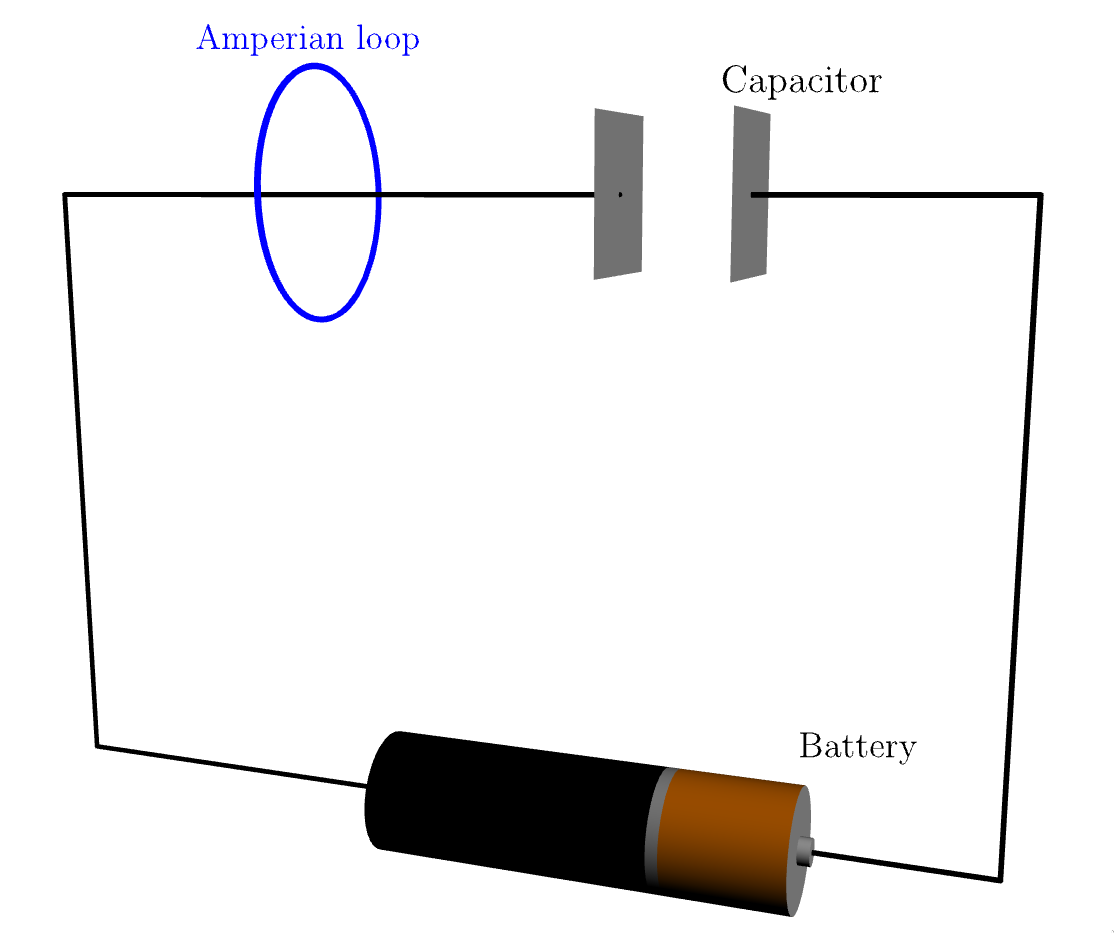
\includegraphics[width=0.5\textheight]{figures/duracell_base.png}
\end{figure}

(The battery is sold separately.)

\end{frame}

\begin{frame}{The Problem with Amp{\'e}re's Law Reveals Itself}

How do we determine $I_{\text{thru}}$? Well, $I_{\text{thru}}$ is the total current passing through the loop. More precisely, \emph{it is the current piercing a surface that has the loop for its boundary}.

\vfill

The simplest surface lies in the plane of the loop:

\begin{figure}[H]
\centering
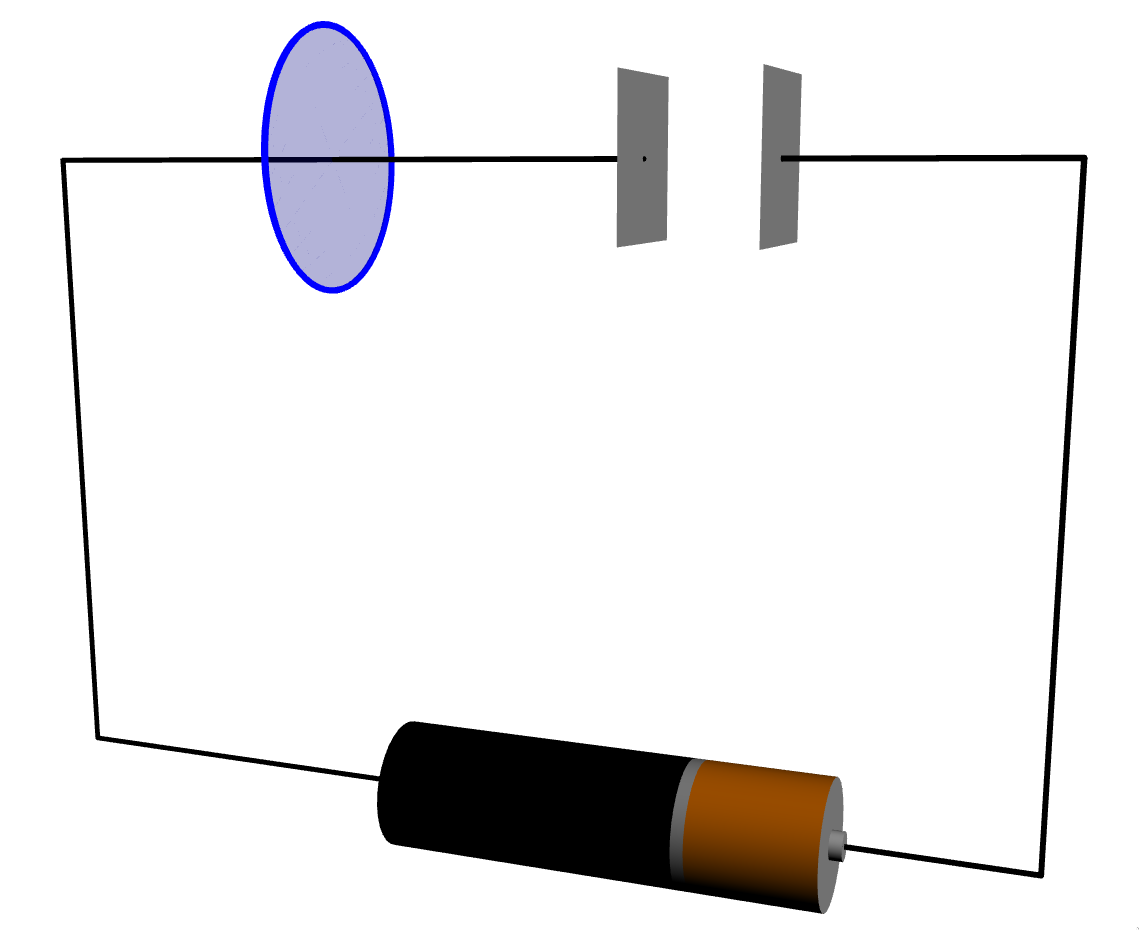
\includegraphics[width=0.5\textheight]{figures/duracell_disk.png}
\end{figure}

\end{frame}

\begin{frame}{The Problem with Amp{\'e}re's Law Reveals Itself}

But we could just as correctly use a balloon-shaped surface:

\begin{figure}[H]
\centering
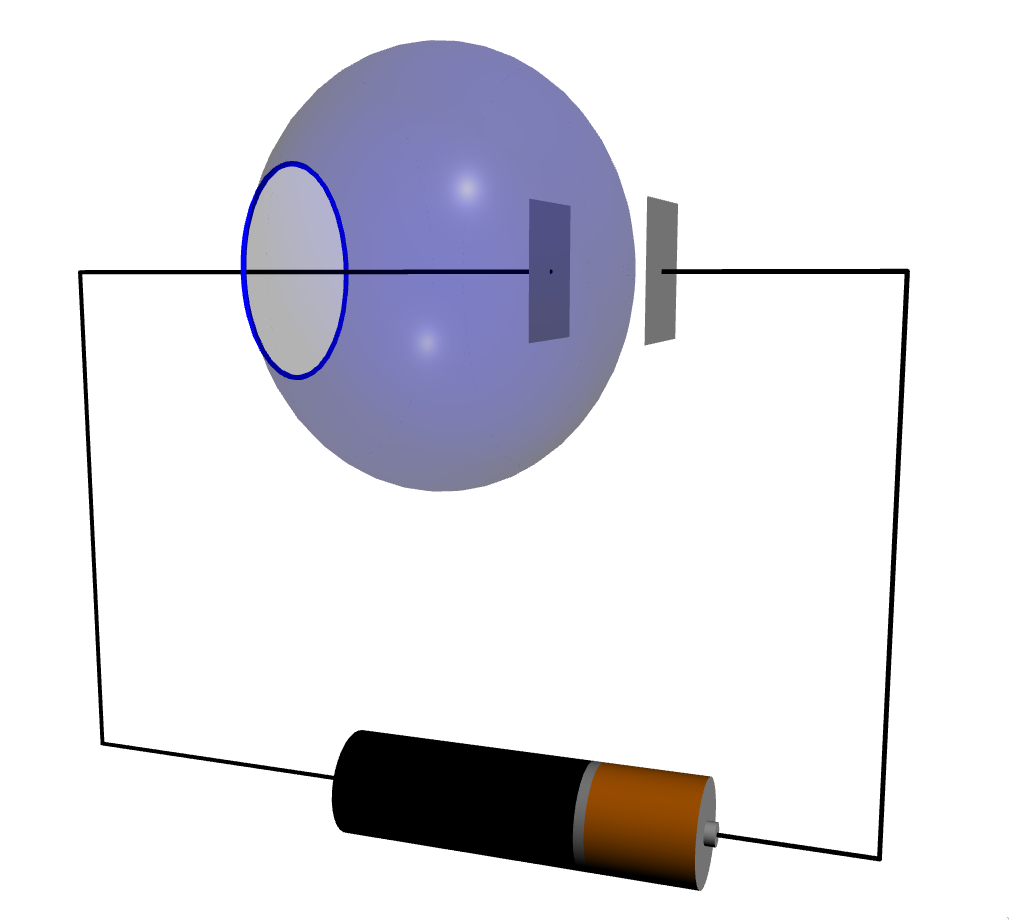
\includegraphics[width=0.5\textheight]{figures/duracell_balloon.png}
\end{figure}

No current passes through \emph{this} surface, and we conclude that $I_{\text{thru}} = 0$! (If this bothers you --- ``obviously one should use the plane surface'' --- remember that the Amperian loop could be some contorted shape that doesn't even lie in a plane)

\end{frame}

\begin{frame}{How Maxwell Fixed Amp{\'e}re's Law}

Maxwell introduced the \emph{displacement current} term into Amp{\'e}re's law that fixes this issue:
\begin{equation*}
    \oint \vec{B} \cdot d\vec{\ell} = \mu_o I_{\text{thru}} + \mu_o \underbrace{\hspace{0.25em}\epsilon_o \frac{d\Phi_E}{dt}\hspace{0.25em}}_{I_{\text{disp}}}
\end{equation*}

It's a misleading name: displacement current has nothing to do with real current (other than sharing units).

\vfill

But Maxwell's correction to Amp{\'e}re's law introduces a certain aesthetic appeal: just as a changing \emph{magnetic} field induces an \emph{electric} field (Faraday's law), so
\begin{center}
    A changing electric field induces a magnetic field!
\end{center}

\end{frame}

\begin{frame}{Classical Electrodynamics}

Altogether, the Maxwell equations are
\begin{equation*}
    \begin{rcases} \displaystyle \oint \vec{E} \cdot d\vec{A} = \frac{Q_{\text{enc}}}{\epsilon_o} & \text{Gauss's law} \\[0.1em] \displaystyle \oint \vec{B} \cdot d\vec{A} = 0 & \text{} \\[0.1em] \displaystyle \oint \vec{E} \cdot d\vec{\ell} = - \int \frac{\partial \vec{B}}{\partial t} \cdot d\vec{A} & \text{Faraday's law} \\[0.1em] \displaystyle \oint \vec{B} \cdot d\vec{\ell} = \mu_o I_{\text{thru}} + \mu_o \epsilon_o \frac{d\Phi_E}{dt} & \text{Amp{\'e}re's law} \end{rcases}
\end{equation*}

The Maxwell equations, together with the Lorentz force law,
\begin{equation*}
    \vec{F} = q \left( \vec{E} + \vec{v} \times \vec{B} \right),
\end{equation*}

form the entire theoretical content of classical electrodynamics! Literally everything we've done in this course has been working out the details of these equations :)

\end{frame}

\begin{frame}{A Primer on Waves}

What is a wave? Here's one working definition: a wave is a disturbance of a continuous medium that propagates with fixed shape at constant velocity.

\vfill

Vague as that may be, it's enough to get us started. But how do we represent that mathematically?

\vfill

Let's turn to the wave equation:
\begin{equation*}
    \frac{\partial^2 g}{\partial z^2} = \frac{1}{v^2} \frac{\partial^2 g}{\partial t^2}
\end{equation*}

\end{frame}

\begin{frame}{The Wave Equation and Sinusoidal Waves}

The wave equation looks kind of scary:
\begin{equation*}
    \frac{\partial^2 g}{\partial z^2} = \frac{1}{v^2} \frac{\partial^2 g}{\partial t^2}
\end{equation*}

And indeed, the wave equation admits all kinds of solutions. But all we really have to worry about is the sinusoidal wave:

\begin{figure}[H]
\centering
\begin{tikzpicture}[scale=1]
    \draw[BLACK, ->] (-4,0) -- (4,0) node[BLACK, anchor=west] {$z$};
    \draw[BLACK, ->] (0,-1.4) -- (0,1.4) node[BLACK, anchor=south] {$g$};
    \draw[BLUE, thick] (-4,1) cos (-3,0);
    \draw[BLUE, thick] (-3,0) sin (-2,-1);
    \draw[BLUE, thick] (-2,-1) cos (-1,0);
    \draw[BLUE, thick] (-1,0) sin (0,1);
    \draw[BLUE, thick] (0,1) cos (1,0);
    \draw[BLUE, thick] (1,0) sin (2,-1);
    \draw[BLUE, thick] (2,-1) cos (3,0);
    \draw[BLUE, thick] (3,0) sin (4,1);
\end{tikzpicture}
\end{figure}

\end{frame}

\begin{frame}{Sinusoidal Waves and Some Terminology}

The most general form of a sinusoidal wave is
\begin{equation*}
    g(z,t) = A \cos{\left[ k\left(z - vt \right) + \delta \right]}
\end{equation*}

Shown below is the plot of the wave above at $t=0$.

\begin{figure}[H]
\centering
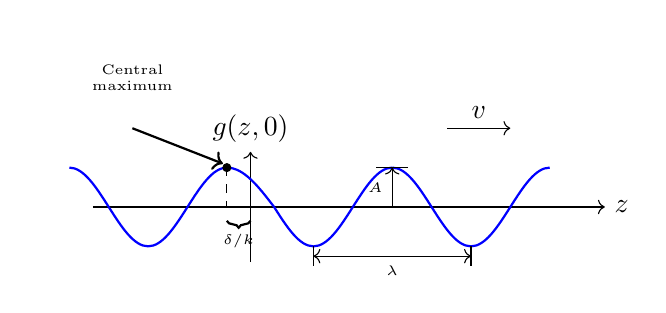
\begin{tikzpicture}[scale=0.5]
    \draw[BLACK, ->] (-4,0) -- (9,0) node[BLACK, anchor=west] {$z$};
    \draw[BLACK, ->] (0,-1.4) -- (0,1.4) node[BLACK, anchor=south] {$g(z,0)$};
    \draw[BLUE, thick] (-4.6,1) cos (-3.6,0);
    \draw[BLUE, thick] (-3.6,0) sin (-2.6,-1);
    \draw[BLUE, thick] (-2.6,-1) cos (-1.6,0);
    \draw[BLUE, thick] (-1.6,0) sin (-0.6,1);
    \draw[BLUE, thick] (-0.6,1) cos (0.6,0);
    \draw[BLUE, thick] (0.6,0) sin (1.6,-1);
    \draw[BLUE, thick] (1.6,-1) cos (2.6,0);
    \draw[BLUE, thick] (2.6,0) sin (3.6,1);
    \draw[BLUE, thick] (3.6,1) cos (4.6,0);
    \draw[BLUE, thick] (4.6,0) sin (5.6,-1);
    \draw[BLUE, thick] (5.6,-1) cos (6.6,0);
    \draw[BLUE, thick] (6.6,0) sin (7.6,1);
    %
    \draw[BLACK, ->] (3.6,0) -- (3.6,1) node[BLACK, left, midway] {\tiny $A$};
    \draw[BLACK] (3.2,1) -- (4.0,1);
    %
    \filldraw[BLACK] (-0.6,1) circle (0.1);
    \node[BLACK, above] at (-3,2) {\parbox[c]{0.2\textwidth}{\begin{center} \tiny Central \\ maximum \end{center}}};
    \draw[BLACK, thick, <-] (-0.7,1.1) -- (-3,2);
    %
    \draw[BLACK, dashed] (-0.6,1) -- (-0.6,0);
	\draw[BLACK, thick, decoration={brace, mirror, raise=5pt}, decorate] (-0.6,0) -- (0,0) node[black, midway, below=6pt] {\tiny $\delta/k$};
	%
	\draw[BLACK, ->] (5,2) -- (6.6,2) node[BLACK, midway, above] {$v$};
	%
	\draw[BLACK] (1.6,-1) -- (1.6,-1.5);
	\draw[BLACK] (5.6,-1) -- (5.6,-1.5);
	\draw[BLACK, <->] (1.6,-1.25) -- (5.6,-1.25) node[BLACK, midway, below] {\tiny $\lambda$};
\end{tikzpicture}
\end{figure}

$A$ is the \emph{amplitude} of the wave, the argument of the cosine is called the \emph{phase}, and $\delta$ is the \emph{phase constant}. Finally, $k$ is the \emph{wave number}; it is related to the wavelength via
\begin{equation*}
	\lambda = 2\pi / k
\end{equation*}

for when $z$ advances by $2\pi/k$, the cosine does one complete cycle.

\end{frame}

\begin{frame}{Sinusoidal Waves and Some More Terminology}

As time passes, the entire wave proceeds to the right, at speed $v$. At any fixed point $z$, the string vibrates up and down, undergoing one full cycle in a period:
\begin{equation*}
	T = \frac{2\pi}{kv}
\end{equation*}

The frequency $f$ (number of oscillations per unit time) is
\begin{equation*}
	f = \frac{1}{T} = \frac{kv}{2\pi} = \frac{v}{\lambda}
\end{equation*}

For our purposes, a more convenient unit is the \emph{angular frequency} $\omega$:
\begin{equation*}
	\omega = 2\pi f = kv
\end{equation*}

Ordinarily, it's nicer to write sinusoidal waves in terms of $\omega$, rather than $v$:
\begin{equation*}
	g(z,t) = A \cos{\left( kz - \omega t + \delta \right)}
\end{equation*}

\end{frame}

\begin{frame}{Maxwell's Equations in a Vacuum}

In a vacuum, there cannot be any charge or current, so Maxwell's equations simplify to
\begin{equation*}
    \begin{cases} \displaystyle \oint \vec{E} \cdot d\vec{A} = 0 \quad \implies \quad \nabla \cdot \vec{E} = 0 \\[1.0em] \displaystyle \oint \vec{B} \cdot d\vec{A} = 0 \quad \implies \quad \nabla \cdot \vec{B} = 0 \\[1.0em] \displaystyle \oint \vec{E} \cdot d\vec{\ell} = - \int \frac{\partial \vec{B}}{\partial t} \cdot d\vec{A} \quad \implies \quad \nabla \times \vec{E} = -\frac{\partial \vec{B}}{\partial t} \\[1.0em] \displaystyle \oint \vec{B} \cdot d\vec{\ell} = \mu_o \epsilon_o \int \frac{\partial \vec{E}}{\partial t} \cdot d\vec{A} \quad \implies \quad \nabla \times \vec{B} = \mu_o \epsilon_o \frac{\partial \vec{E}}{\partial t} \end{cases}
\end{equation*}

(The equations on the right are known as the Maxwell equations in differential form --- they are completely equivalent to their integral counterparts).

\end{frame}

\begin{frame}{The Wave Nature of Light}

A little bit of math on the previous equations gets us
\begin{equation*}
	\nabla^2 \vec{E} = \mu_o \epsilon_o \frac{\partial^2 \vec{E}}{\partial t^2}, \qquad \nabla^2 \vec{B} = \mu_o \epsilon_o \frac{\partial^2 \vec{B}}{\partial t^2}
\end{equation*}

Look at that! That takes the same form as the wave equation in 3D:
\begin{equation*}
	\nabla^2 g = \frac{1}{v^2} \frac{\partial^2 g}{\partial t^2}
\end{equation*}

This tells us that in a vacuum, light propagates as a wave, with speed
\begin{equation*}
	v = \frac{1}{\sqrt{\epsilon_o \mu_o}} = c = \SI{3.00e8}{\metre/\second}
\end{equation*}

\end{frame}

\begin{frame}{Monochromatic Plane Waves}

Again we'll confine our attention to sinusoidal waves of frequency $\omega$. Since different frequencies in the visible range correspond to different colors, such waves are called \emph{monochromatic}.

\begin{columns}

\column{0.60\textwidth}
\begin{figure}[H]
\centering
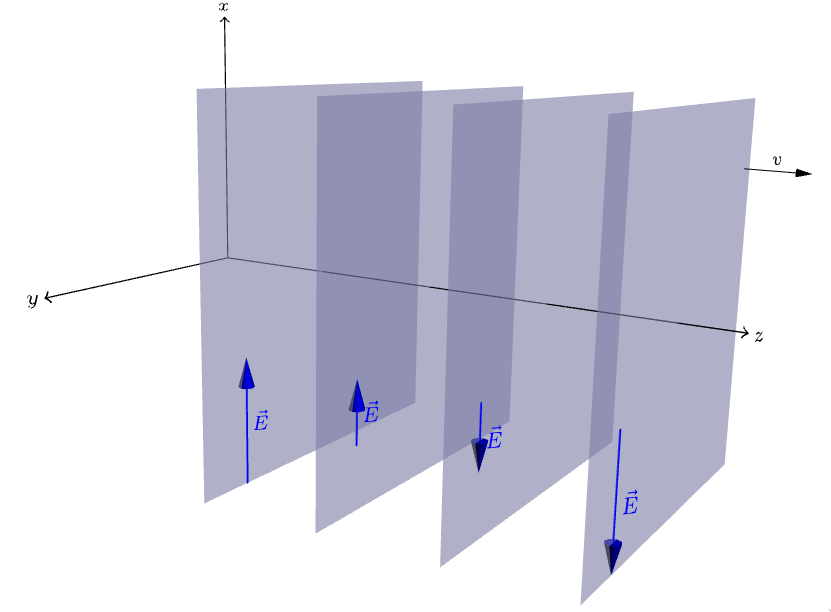
\includegraphics[height=0.50\textheight]{figures/plane_wave.png}
\end{figure}

\column{0.4\textwidth}
Suppose, moreover, that the waves are traveling in the $z$ direction and have no $x$ or $y$ dependence; these are called \emph{plane waves}, because the fields are uniform over every plane perpendicular to the direction of propagation.

\end{columns}

\end{frame}

\begin{frame}{Electromagnetic Waves are Transverse}

Electromagnetic waves are \emph{transverse}: the electric and magnetic fields are perpendicular to the direction of propagation.

\vfill

Moreover, $\vec{E}$ and $\vec{B}$ are \emph{in phase and mutually perpendicular}; their amplitudes are related by
\begin{equation*}
    B_o = \frac{k}{\omega} E_o = \frac{1}{c} E_o
\end{equation*}

\end{frame}

\begin{frame}{Electromagnetic Waves Visualized}

Take the following wave, for example. It is propagating in the positive $z$ direction, with $\vec{E}$ pointing in the $x$ direction, and $\vec{B}$ pointing in the $y$ direction.

\vspace{-0.4em}

\begin{figure}[H]
\centering
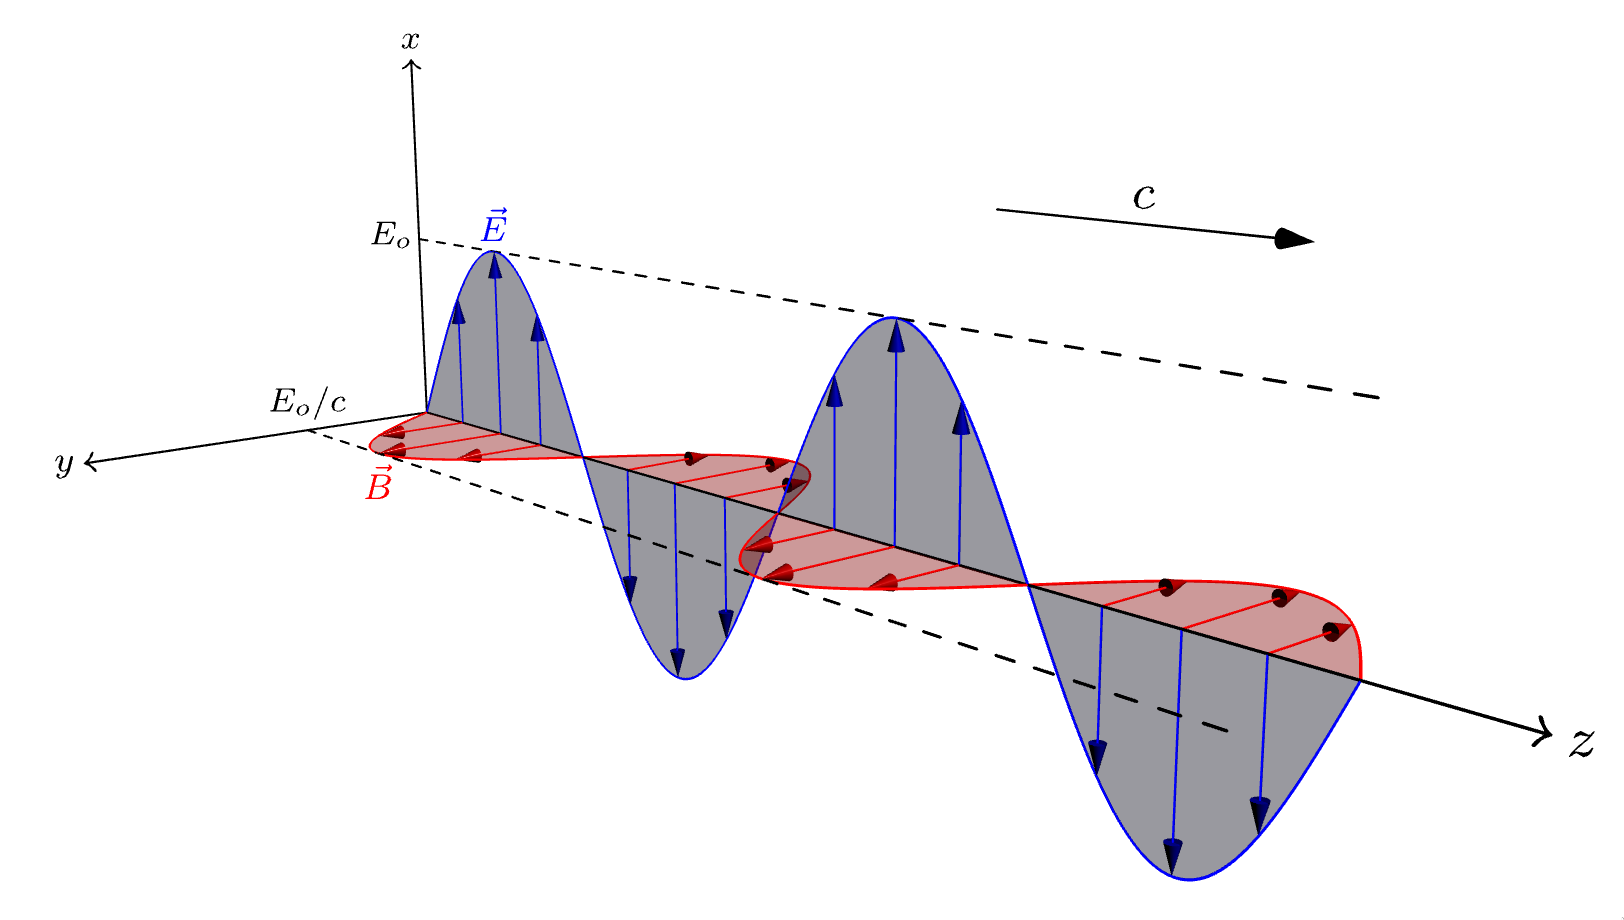
\includegraphics[width=0.8\textwidth]{figures/em_wave.png}
\end{figure}

\vspace{-1.6em}

The electric and magnetic fields are given by
\begin{gather*}
    \vec{E} (z, t) = E_o \cos{\left( kz - \omega t + \delta \right)} \ihat, \\
    \vec{B} (z, t) = \frac{1}{c} E_o \cos{\left( kz - \omega t + \delta \right)} \jhat
\end{gather*}

\end{frame}

\begin{frame}{Energy in Electromagnetic Fields}

When studying electrostatics, we determined that the work necessary to assemble a static charge distribution (against the Coulomb repulsion of like charges) is
\begin{equation*}
    W_e = \frac{\epsilon_o}{2} \int E^2 dV
\end{equation*}

where $\vec{E}$ is the resulting electric field. Likewise, the work required to get currents going (against the back emf) is
\begin{equation*}
    W_m = \frac{1}{2\mu_o} \int B^2 dV
\end{equation*}

where $\vec{B}$ is the resulting magnetic field. This suggests that the total energy stored in electromagnetic fields, per unit volume, is
\begin{equation*}
    u = \underbrace{\hspace{0.5em}\frac{1}{2}\epsilon_o E^2\hspace{0.5em}}_{u_e} + \underbrace{\hspace{0.5em}\frac{1}{2\mu_o} B^2\hspace{0.5em}}_{u_m} = \frac{1}{2} \left( \epsilon_o E^2 + \frac{1}{\mu_o} B^2 \right)
\end{equation*}

\end{frame}

\begin{frame}{The Poynting Vector}

The \emph{energy per unit time, per unit area,} transported by electromagnetic fields is called the Poynting vector:
\begin{equation*}
    S \equiv \frac{1}{\mu_o} \left( \vec{E} \times \vec{B} \right)
\end{equation*}

Specifically, $\vec{S} \cdot d\vec{A}$ is the energy per unit time crossing the infinitesimal surface $d\vec{A}$ --- the energy \emph{flux} (so $\vec{S}$ is the \emph{energy flux density}).

\end{frame}

\begin{frame}{Concerning Energy and Momentum in Electromagnetic Waves --- What's Coming Up}

The next 5 slides are a derivation of frequently used equations that concern energy and momentum in electromagnetic waves.

\vfill

The derivations are a little math-heavy, but are nonetheless insightful.

\end{frame}

\begin{frame}{Energy \& Momentum in Electromagnetic Waves (Part 1)}

Suppose we have a monochomatic plane wave propagating in the positive $z$ direction (such as the one shown a few slides back). It's electric and magnetic fields are described by
\begin{gather*}
    \vec{E} (z, t) = E_o \cos{\left( kz - \omega t + \delta \right)} \ihat, \\
    \vec{B} (z, t) = \frac{1}{c} E_o \cos{\left( kz - \omega t + \delta \right)} \jhat
\end{gather*}

Since $E = cB$, the energy per unit volume is
\begin{gather*}
    u = \frac{1}{2} \left( \epsilon_o E^2 + \frac{1}{\mu_o} B^2 \right) = \frac{1}{2} \left( \epsilon_o E^2 \frac{1}{\cancel{\mu_o}} \cancel{\mu_o} \epsilon_o E^2 \right) \\
    \implies u = \epsilon_o E^2 = \epsilon_o E_o^2 \cos^2{\left( kz - \omega t + \delta \right)}
\end{gather*}

\end{frame}

\begin{frame}{Energy \& Momentum in Electromagnetic Waves (Part 2)}

Now let's calculate the Poynting vector for the same monochromatic plane wave:
\begin{gather*}
    \vec{S} = \frac{1}{\mu_o} \left( \vec{E} \times \vec{B} \right) = \frac{1}{\mu_o} \frac{E_o^2}{c} \cos^2{\left( kz - \omega t + \delta \right)} \khat \\
    \implies \vec{S} = c \underbrace{\epsilon_o E_o^2 \cos^2{\left( kz - \omega t + \delta \right)}}_{u} \khat
\end{gather*}

Notice that $\vec{S}$ is the energy density ($u$) times the velocity of the waves ($c \khat$) --- as it should be. After all, in a time $\Delta t$, a length $c\ \Delta t$ passes through an area $A$, carrying with it an energy $u A c\ \Delta t$. The energy per unit time, per unit area, transported by the wave is therefore $uc$.

\vfill

(To compute the cross-product, note that $\vec{E}$ and $\vec{B}$ are perpendicular, so $\ihat \times \jhat = \khat$. Also, observe that $\frac{1}{\mu_o c} = c \epsilon_o$.)

\end{frame}

\begin{frame}{Energy \& Momentum in Electromagnetic Waves (Part 3)}

So far, we have that for a monochromatic plane wave, the Poynting vector is $\vec{S} = c \epsilon_o E_o^2 \cos^2{\left( kz - \omega t + \delta \right)}\ \khat$. But in the case of light, the wavelength is so short and the period is so brief that any measurement will encompass many cycles. Typically, therefore, we want the average value. The average of cosine-squared over a complete cycle is
\begin{equation*}
    \frac{1}{T} \int_0^T \cos^2{\left( kz - \frac{2\pi t}{T} + \delta \right)}\ dt = \frac{1}{2}
\end{equation*}

So we have
\begin{equation*}
    \langle \vec{S} \rangle = \frac{1}{2} c \epsilon_o E_o^2\ \khat
\end{equation*}

Where the brackets, $\langle\ \rangle$, denote the time average over a complete cycle. The average power per unit area transported by an electromagnetic wave is called the \emph{intensity}:
\begin{equation*}
    I \equiv \langle S \rangle = \frac{1}{2} c \epsilon_o E_o^2 = \frac{P_{\text{avg}}}{A}
\end{equation*}

\end{frame}

\begin{frame}{Energy \& Momentum in Electromagnetic Waves (Part 4)}

Electromagnetic fields not only carry energy, they also carry momentum. The momentum density (analogous to the energy density) stored in the field is
\begin{equation*}
    \vec{g} = \frac{1}{c^2} \vec{S}
\end{equation*}

For monochomatic plane waves, then,
\begin{equation*}
    \vec{g} = \frac{1}{c} \epsilon_o E_o^2 \cos^2{\left( kz - \omega t + \delta \right)}\ \khat = \frac{1}{c} u\ \khat
\end{equation*}

As before, the average value over a complete cycle is
\begin{equation*}
    \langle \vec{g} \rangle = \frac{1}{2c} \epsilon_o E_o^2\ \khat
\end{equation*}

\end{frame}

\begin{frame}{Energy \& Momentum in Electromagnetic Waves (Part 5)}

When light falls (at normal incidence) on a perfect absorber, it delivers its momentum to the surface. In a time $\Delta t$, the momentum transfer is $\Delta \vec{p} = \langle \vec{g} \rangle A c\ \Delta t$, so the \emph{radiation pressure} (average force per unit area) is
\begin{equation*}
    \mathscr{P} = \frac{1}{A} \frac{\Delta p}{\Delta t} = \frac{1}{2} \epsilon_o E_o^2 = \frac{I}{c}
\end{equation*}

On a perfect reflector, the pressure is twice as great.

\end{frame}

\begin{frame}{Energy and Momentum in Electromagnetic Waves Summarized}


We're done with the derivations! Here's a quick summary of what we've learned.

\vfill

Electromagnetic waves carry both energy and momentum.

\vfill

The intensity of an electromagnetic wave (average power per unit area) is:
\begin{equation*}
    I = \frac{1}{2} c \epsilon_o E_o^2 = \frac{P_{\text{avg}}}{A}
\end{equation*}

Remember! Often we deal with light sources that propagate outwards (into a sphere, for instance). We would take the area to be $4\pi r^2$ for a sphere, $2\pi r^2$ for a hemisphere, etc.

\end{frame}

\begin{frame}{Energy and Momentum in Electromagnetic Waves Summarized}

For a perfect absorber, the radiation pressure (average force per unit area) is:
\begin{equation*}
    \mathscr{P} = \frac{1}{A} \frac{\Delta p}{\Delta t} = \frac{1}{2} \epsilon_o E_o^2 = \frac{I}{c}
\end{equation*}

And for a perfect reflector, the radiation pressure is $\frac{2I}{c}$ --- twice as great.

\vfill

Wow that's a bunch of p's. Here's how I recommend not getting confused:
\begin{equation*}
    \begin{cases} \text{Momentum} \ \to \ p \text{ (lowercase)} \\ \text{Power} \ \to \ P \text{ (uppercase)} \\ \text{Radiation pressure} \ \to \ \mathscr{P} \text{ (or some special p)} \end{cases}
\end{equation*}

\end{frame}

\begin{frame}{Geometric Optics --- Reflection}

Light coming into a surface bounces off (reflects) the surface at the same angle (defined relative to the normal) that it came in at:

\begin{equation*}
    \theta_{\text{incident}} = \theta_{\text{reflect}}
\end{equation*}

\begin{figure}[H]
\centering
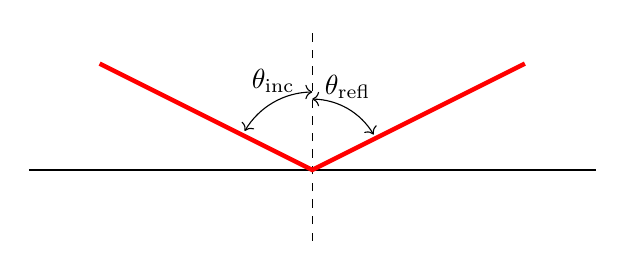
\begin{tikzpicture}[scale=0.9]
    \draw[BLACK, thick] (-4,0) -- (4,0);
    \draw[BLACK, dashed] (0,-1) -- (0,2);
    \draw[RED, ultra thick] (-3,1.5) -- (0,0) -- (3,1.5);
    \draw[BLACK, <->] (0,1.1) arc (90:150:1.1) node[BLACK, midway, anchor=south] {$\theta_{\text{inc}}$};
    \draw[BLACK, <->] (0,1) arc (90:30:1) node[BLACK, midway, anchor=south] {$\theta_{\text{refl}}$};
\end{tikzpicture}
\end{figure}

\end{frame}

\begin{frame}{Geometric Optics --- Refraction}

Light going from one material to another, it bends (refracts) according to Snell's law:

\begin{equation*}
    n_1 \sin{\theta_1} = n_2 \sin{\theta_2}
\end{equation*}

\begin{figure}[H]
\centering
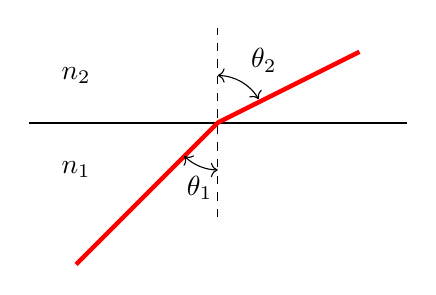
\begin{tikzpicture}[scale=0.6]
    \draw[BLACK, thick] (-4,0) -- (4,0);
    \draw[BLACK, dashed] (0,-2) -- (0,2);
    \draw[RED, ultra thick] (-3,-3) -- (0,0) -- (3,1.5);
    \draw[BLACK, <->] (0,-1) arc (270:225:1) node[BLACK, midway, anchor=north] {$\theta_1$};
    \draw[BLACK, <->] (0,1) arc (90:30:1) node[BLACK, midway, anchor=south west] {$\theta_2$};
    \node[BLACK] at (-3,-1) {$n_1$};
    \node[BLACK] at (-3,1) {$n_2$};
\end{tikzpicture}
\end{figure}

The \emph{index of refraction} is a property of the material:
\begin{equation*}
    n = \frac{c}{v} > 1
\end{equation*}

For a vacuum, the index of refraction is defined to be 1. In a material, the index of refraction is greater than 1.

\end{frame}

\begin{frame}{Geometric Optics --- Total Internal Reflection}

Suppose at refraction angle $\theta_2$ is \ang{90}. Then the light is completely confined to the first material: it undergoes \emph{total internal reflection}!

\vspace{-2em}

\begin{figure}[H]
\centering
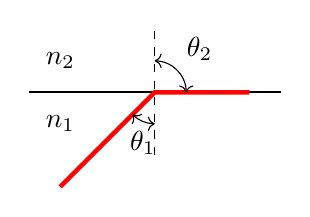
\begin{tikzpicture}[scale=0.4]
    \draw[BLACK, thick] (-4,0) -- (4,0);
    \draw[BLACK, dashed] (0,-2) -- (0,2);
    \draw[RED, ultra thick] (-3,-3) -- (0,0) -- (3,0);
    \draw[BLACK, <->] (0,-1) arc (270:225:1) node[BLACK, midway, anchor=north] {$\theta_1$};
    \draw[BLACK, <->] (0,1) arc (90:0:1) node[BLACK, midway, anchor=south west] {$\theta_2$};
    \node[BLACK] at (-3,-1) {$n_1$};
    \node[BLACK] at (-3,1) {$n_2$};
\end{tikzpicture}
\end{figure}

\vspace{-1em}

Then $\theta_1$, the incident angle, is known as the \emph{critical angle}. This critical angle is
\begin{equation*}
    n_1 \sin{\theta_1} = n_2 \cancelto{1}{\sin{90}} \quad \implies \quad \theta_1 = \theta_c = \sin^{-1}{\left( \frac{n_2}{n_1} \right)}
\end{equation*}

Note that the inverse sine function $\sin^{-1}{x}$ is not defined for $x > 1$. Then it follows that $n_1 > n_2$. That is, in order for TIR to occur, the light must be within a medium with a higher index of refraction than its surroundings.

\end{frame}

\begin{frame}{Physical Optics}

The key idea of physical optics is to consider the wave-like nature of light.

\vfill

Constructive interference occurs when the path length difference is an integer multiple of the wavelength:
\begin{equation*}
    \Delta r = r_2 - r_1 = m \lambda
\end{equation*}

Destructive interference occurs when the path length difference is a half-integer multiple of the wavelength:
\begin{equation*}
    \Delta r = r_2 - r_1 = \left( m + \frac{1}{2} \right) \lambda
\end{equation*}

\end{frame}

\begin{frame}{Physical Optics --- Bragg Diffraction}

The governing equation for Bragg Diffraction is
\begin{equation*}
    d\sin{\theta_{\text{inc}}} + d\sin{\theta_{\text{ref}}} = m \lambda
\end{equation*}

Or, if the incident angle is the same as the reflected angle,
\begin{equation*}
    2d\sin{\theta} = m \lambda
\end{equation*}

This is nothing more than a constructive interference condition.

\end{frame}

\end{document}
